%!Mode:: "TeX:UTF-8"
\documentclass[a4paper,11pt,UTF8]{ctexart}

\usepackage{indentfirst} %缩进
\usepackage{xeCJK}    %使用系统字体
\usepackage{fancyhdr} %自定义页眉页脚
\pagestyle{empty}                   %不设置页眉页脚
\usepackage{amsmath, amsthm, amssymb, amsfonts} %数学公式
\usepackage[a4paper,left=3cm,right=3cm,top=3cm,bottom=3cm]{geometry}
%\usepackage[tmargin=1in,bmargin=1in,lmargin=1.25in,rmargin=1.25in]{geometry}.
\usepackage{booktabs} %插入表格
\usepackage[section]{placeins} %避免浮动
\usepackage{listings} %插入代码
\usepackage{ctex}     %中文宏包
\usepackage[svgnames, table]{xcolor} %彩色表格
\usepackage{algorithm}          %伪代码
\usepackage{algorithmicx}
\usepackage{algpseudocode}
\usepackage{algorithm,algpseudocode,float}
\usepackage{lipsum}
\usepackage{enumitem}           %调整列举环境
\usepackage{url}
\usepackage{fontspec,xunicode}
\defaultfontfeatures{Mapping=tex-text} %如果没有它,会有一些 tex 特殊字符无法正常使用,比如连字符。
\usepackage{subcaption}
\usepackage{graphicx}
\graphicspath{{imgs/}}

%%%%%%%%%%%%%%%%%%%%%%%%%%%%%%%%%%%%%%%%%%%%%%%%%%%%%%%%%%%%%%%%
% 缩进及行间距
%%%%%%%%%%%%%%%%%%%%%%%%%%%%%%%%%%%%%%%%%%%%%%%%%%%%%%%%%%%%%%%%
\setlength{\parindent}{22pt} %重新定义缩进长度
\setlength{\baselineskip}{20pt}  %定义行间距
%\renewcommand{\baselinestretch}{1.1} %定义行间距

%%%%%%%%%%%%%%%%%%%%%%%%%%%%%%%%%%%%%%%%%%%%%%%%%%%%%%%%%%%%%%%%
% 列表设置
%%%%%%%%%%%%%%%%%%%%%%%%%%%%%%%%%%%%%%%%%%%%%%%%%%%%%%%%%%%%%%%%
\setenumerate{fullwidth,itemindent=\parindent,listparindent=\parindent,itemsep=0ex,partopsep=0pt,parsep=0ex}
\setenumerate[2]{label=\alph*),leftmargin=1.5em}  %二级item设置
\setitemize{itemindent=38pt,leftmargin=0pt,itemsep=-0.4ex,listparindent=26pt,partopsep=0pt,parsep=0.5ex,topsep=-0.25ex}
\setdescription{itemindent=38pt,leftmargin=0pt,itemsep=-0.4ex,listparindent=26pt,partopsep=0pt,parsep=0.5ex,topsep=-0.25ex}

%%%%%%%%%%%%%%%%%%%%%%%%%%%%%%%%%%%%%%%%%%%%%%%%%%%%%%%%%%%%%%%%
% 图的标题行间距设置
%%%%%%%%%%%%%%%%%%%%%%%%%%%%%%%%%%%%%%%%%%%%%%%%%%%%%%%%%%%%%%%%
\newcommand{\bottomcaption}{%
\setlength{\abovecaptionskip}{6pt}%
\setlength{\belowcaptionskip}{6pt}%
\caption}


%%%%%%%%%%%%%%%%%%%%%%%%%%%%%%%%%%%%%%%%%%%%%%%%%%%%%%%%%%%%%%%%
% 字体定义
%%%%%%%%%%%%%%%%%%%%%%%%%%%%%%%%%%%%%%%%%%%%%%%%%%%%%%%%%%%%%%%%
\setmainfont{Times New Roman}  %默认英文字体.serif是有衬线字体sans serif无衬线字体
\setmonofont{Consolas}
\setCJKmainfont[ItalicFont={楷体}, BoldFont={黑体}]{宋体}%衬线字体 缺省中文字体为
\setCJKsansfont{黑体}
\punctstyle{hangmobanjiao}
%-----------------------xeCJK下设置中文字体------------------------------%
\setCJKfamilyfont{song}{SimSun}                             %宋体 song
\newcommand{\song}{\CJKfamily{song}}
\setCJKfamilyfont{fs}{FangSong}                      %仿宋  fs
\newcommand{\fs}{\CJKfamily{fs}}
\setCJKfamilyfont{ktgb}{KaiTi}                      %楷体2312 ktgb
\newcommand{\ktgb}{\CJKfamily{ktgb}}
\setCJKfamilyfont{yh}{Microsoft YaHei}                    %微软雅黑 yh
\newcommand{\yh}{\CJKfamily{yh}}
\setCJKfamilyfont{hei}{SimHei}                              %黑体  hei
\newcommand{\hei}{\CJKfamily{hei}}
\setCJKfamilyfont{hwxk}{STXingkai}                                %华文行楷  hwxk
\newcommand{\hwxk}{\CJKfamily{hwxk}}
%------------------------------设置字体大小------------------------%
\newcommand{\shiyanbaogao}{\fontsize{36pt}{\baselineskip}\selectfont}
\newcommand{\chuhao}{\fontsize{42pt}{\baselineskip}\selectfont}     %初号
\newcommand{\xiaochuhao}{\fontsize{36pt}{\baselineskip}\selectfont} %小初号
\newcommand{\yihao}{\fontsize{28pt}{\baselineskip}\selectfont}      %一号
\newcommand{\erhao}{\fontsize{21pt}{\baselineskip}\selectfont}      %二号
\newcommand{\xiaoerhao}{\fontsize{18pt}{\baselineskip}\selectfont}  %小二号
\newcommand{\sanhao}{\fontsize{15.75pt}{\baselineskip}\selectfont}  %三号
\newcommand{\sihao}{\fontsize{14pt}{\baselineskip}\selectfont}       %四号
\newcommand{\xiaosihao}{\fontsize{12pt}{\baselineskip}\selectfont}  %小四号
\newcommand{\wuhao}{\fontsize{10.5pt}{\baselineskip}\selectfont}    %五号
\newcommand{\xiaowuhao}{\fontsize{9pt}{\baselineskip}\selectfont}   %小五号
\newcommand{\liuhao}{\fontsize{7.875pt}{\baselineskip}\selectfont}  %六号
\newcommand{\qihao}{\fontsize{5.25pt}{\baselineskip}\selectfont}    %七号

%%%%%%%%%%%%%%%%%%%%%%%%%%%%%%%%%%%%%%%%%%%%%%%%%%%%%%%%%%%%%%%%
% 图题字体大小相同
%%%%%%%%%%%%%%%%%%%%%%%%%%%%%%%%%%%%%%%%%%%%%%%%%%%%%%%%%%%%%%%%
\usepackage{caption}
\captionsetup{font={footnotesize}}   % footnotesize = 9pt
\captionsetup[lstlisting]{font={footnotesize}}

%%%%%%%%%%%%%%%%%%%%%%%%%%%%%%%%%%%%%%%%%%%%%%%%%%%%%%%%%%%%%%%%
% 重定义枚举编号为 1),2)...
%%%%%%%%%%%%%%%%%%%%%%%%%%%%%%%%%%%%%%%%%%%%%%%%%%%%%%%%%%%%%%%%
\renewcommand{\labelenumi}{\theenumi}


%%%%%%%%%%%%%%%%%%%%%%%%%%%%%%%%%%%%%%%%%%%%%%%%%%%%%%%%%%%%%%%%
% 重定义section标题
%%%%%%%%%%%%%%%%%%%%%%%%%%%%%%%%%%%%%%%%%%%%%%%%%%%%%%%%%%%%%%%%
\CTEXsetup[format={\sihao\CJKfamily{zhhei}\zihao{4}},number={\chinese{section}},name={,、~},aftername={},indent={0pt},beforeskip={6pt},afterskip={6pt},format+={\flushleft}]{section}
\CTEXsetup[number={\chinese{section}},name={附录, ~~ }]{appendix}



%%%%%%%%%%%%%%%%%%%%%%%%%%%%%%%%%%%%%%%%%%%%%%%%%%%%%%%%%%%%%%%%
% 标题名称中文化
%%%%%%%%%%%%%%%%%%%%%%%%%%%%%%%%%%%%%%%%%%%%%%%%%%%%%%%%%%%%%%%%
\renewcommand\figurename{\hei 图}
\renewcommand\tablename{\hei 表}
\renewcommand\lstlistingname{\hei 代码}
\renewcommand{\algorithmicrequire}{\textbf{输入:}}
\renewcommand{\algorithmicensure}{\textbf{输出:}}
\newtheorem{define}{定义}

%%%%%%%%%%%%%%%%%%%%%%%%%%%%%%%%%%%%%%%%%%%%%%%%%%%%%%%%%%%%%%%%
% 代码设置
%%%%%%%%%%%%%%%%%%%%%%%%%%%%%%%%%%%%%%%%%%%%%%%%%%%%%%%%%%%%%%%%
\lstset{
 columns=fixed,
 numbers=left,                                        % 在左侧显示行号
 numberstyle=\tiny\color{gray},                       % 设定行号格式
 frame=single,                                        % 单线背景边框
 breaklines=true,                                     % 设定LaTeX对过长的代码行进行自动换行
 keywordstyle=\color[RGB]{40,40,255},                 % 设定关键字颜色
 numberstyle=\footnotesize\color{darkgray},
 commentstyle=\it\color[RGB]{0,96,96},                % 设置代码注释的格式
 stringstyle=\rmfamily\slshape\color[RGB]{128,0,0},   % 设置字符串格式
 showstringspaces=false,                              % 不显示字符串中的空格
 language=java,                                        % 设置语言
 basicstyle=\linespread{1.0}\xiaowuhao\ttfamily,                      % 字体字号
 %lineskip=10pt,
 %baselinestretch=1,
}

%%%%%%%%%%%%%%%%%%%%%%%%%%%%%%%%%%%%%%%%%%%%%%%%%%%%%%%%%%%%%%%%
% 伪代码分页
%%%%%%%%%%%%%%%%%%%%%%%%%%%%%%%%%%%%%%%%%%%%%%%%%%%%%%%%%%%%%%%%
\makeatletter
\renewcommand{\ALG@name}{算法}
\newenvironment{breakablealgorithm}
  {% \begin{breakablealgorithm}
   \begin{center}
     \refstepcounter{algorithm}% New algorithm
     \hrule height.8pt depth0pt \kern2pt% \@fs@pre for \@fs@ruled
     \renewcommand{\caption}[2][\relax]{% Make a new \caption
       {\raggedright\textbf{\ALG@name~\thealgorithm} ##2\par}%
       \ifx\relax##1\relax % #1 is \relax
         \addcontentsline{loa}{algorithm}{\protect\numberline{\thealgorithm}##2}%
       \else % #1 is not \relax
         \addcontentsline{loa}{algorithm}{\protect\numberline{\thealgorithm}##1}%
       \fi
       \kern2pt\hrule\kern2pt
     }
  }{% \end{breakablealgorithm}
     \kern2pt\hrule\relax% \@fs@post for \@fs@ruled
   \end{center}
  }
\makeatother



\begin{document}
\xiaosihao\song

\begin{titlepage}
\center{\yihao{\hwxk{武汉大学国家网络安全学院}}}
\vspace{6cm}
\center{\shiyanbaogao{\ktgb{密~码~学~实~验~报~告}}}
\vspace{4cm}

\begin{center}
\begin{large}
\begin{tabular}{rc}
\xiaoerhao{\hei{学\qquad 号}}& \hspace{1.7cm}\xiaoerhao{\hei{2021302181156\hspace{1.7cm}}} \\
\cline{2-2}\\
\xiaoerhao{\hei{姓\qquad 名}}& \xiaoerhao{\hei{赵~伯~俣}}\\
\cline{2-2}\\
\xiaoerhao{\hei{实验名称}}& \xiaoerhao{\hei{序列密码}}\\
\cline{2-2}\\
\xiaoerhao{\hei{指导教师}}& \xiaoerhao{\hei{何琨}}\\
\cline{2-2}
\end{tabular}
\end{large}
\end{center}
\vfill \hfill
\end{titlepage}
\clearpage

% \centerline{\\[10pt]\erhao{\fs{武 ~汉 ~ 大~ 学}}}
% \centerline{\\[10pt]\yihao{\fs{信~息~隐~藏~实~验~报~告}}}

% \leftline{\\[10pt]\sihao{\hei{\hspace{1.5em} 学生姓名:XXX \hfill 学号:XXXX \hfill 指导教师:XXX }}}

% \leftline{\\[10pt]\sihao{\hei{\hspace{1.5em} 实验地点:新珈楼XXX \hfill }}}

% \leftline{\\[10pt]\sihao{\hei{\hspace{1.5em} 实验时间:第X周周X(X-X节) \hfill }}}



\setlength{\parskip}{6pt}  %定义段间距

\section{实验名称: 序列密码}
\section{实验目的及要求:}

  \subsection{实验目的}
    $(1)$掌握序列密码的基本概念\par
    $(2)$掌握线性移位寄存器的结构及其序列的伪随机性\par
    $(3)$熟悉非线性序列的概念与基本产生方法\par
    $(4)$了解常用伪随机性评价方法\par
    $(5)$掌握一种典型流密码(如RC4或ZUC等)\par

  \subsection{实验要求}
    $(1)$掌握序列密码的实现方案\par
    $(2)$掌握线性移位寄存器的构造\par
    $(3)$熟悉序列伪随机性的基本测试方法\par
    $(4)$实现RC4或ZUC算法\par


\section{实验设备环境及要求:}
  Windows操作系统,python高级语言开发环境

\section{实验内容与步骤:}

  \subsection{序列密码实现方案}
    \subsubsection{种子密钥K输入到密钥流发生器}
      该步骤是序列密码的起始步骤。在这里,一个预先定义的密钥(称为种子密钥K)被输入到一个专门的算法或设备中,
      即密钥流发生器。这个种子密钥通常是一串固定长度的二进制数字,它的作用是为接下来的密钥流生成提供基础。
      种子密钥的选择非常重要,因为它直接影响到生成的密钥流的随机性和安全性。
    \subsubsection{产生一系列密钥流}
      在种子密钥输入之后,密钥流发生器开始产生一个长序列的密钥流。这个密钥流实际上是一个很长的伪随机二进制数字序列,
      它用于后续的加密过程。这个过程的关键在于生成的密钥流必须是高度随机的,以确保加密的安全性。
      密钥流的长度通常取决于明文的长度,以确保每个明文单元都有一个对应的密钥单元。
    \subsubsection{通过与同一时刻的一个字节或者一位明文流进行异或操作产生密文流}
      最后一步是将密钥流与明文数据进行组合。这通常是通过异或(XOR)操作完成的。在异或操作中,
      密钥流中的每一位或字节与明文流中相应的位或字节组合。如果明文和密钥流的相应位相同,则结果为0;
      如果不同,则结果为1。这样生成的序列就是密文流,它可以被发送到接收方。接收方在拥有相同密钥流的前提下,
      可以通过相同的异或操作将密文解密回原始明文。

  \subsection{线性移位寄存器的构造}

    \subsubsection{选择连接多项式(一般选择本原多项式作为连接多项式)}
      连接多项式在LFSR中起着核心作用。它决定了反馈逻辑,从而影响生成的序列的特性。
      本原多项式是一种特殊的多项式,它具有生成最长周期序列的能力。在选择本原多项式时,它能确保LFSR产生的序列具有最大的周期,
      这对于加密应用是非常重要的。
      这些多项式是在有限域上定义的,通常表示为一系列系数,这些系数对应于LFSR中的反馈点。
    \subsubsection{根据连接多项式的反馈系数得出反馈函数}
      反馈函数是LFSR的核心,它定义了如何从当前的寄存器状态生成下一个状态。
      这个函数是基于连接多项式的系数来构建的。这些系数决定了在LFSR中哪些位会被用于计算反馈值。
      反馈函数通常是通过将选定的寄存器位进行异或(XOR)操作来实现的。这些选定的位是由连接多项式的非零系数位置决定的。
    \subsubsection{根据反馈函数得出每个节拍的寄存器状态}
      在LFSR的每个时钟周期(节拍)中,根据反馈函数计算新的输出位,并将其反馈到寄存器的最末端。
      同时,寄存器中的其他位将根据寄存器的工作方式向前移动一位。
      这个过程不断重复,每个新的时钟周期都会根据反馈函数更新寄存器的状态,从而生成一个伪随机序列。

    \subsubsection{实验(1)}
      使用本原多项式$g1(x)=x^{4} +x +1$为连接多项式组成线性移位寄存器。画出逻辑图,写出输出序列及状态变迁。\par
      将本原多项式$g1(x)=x^{4} +x +1$选定为连接多项式得到的线性移位寄存器的逻辑图如下图所示
      \begin{figure}[H]
        \centering
        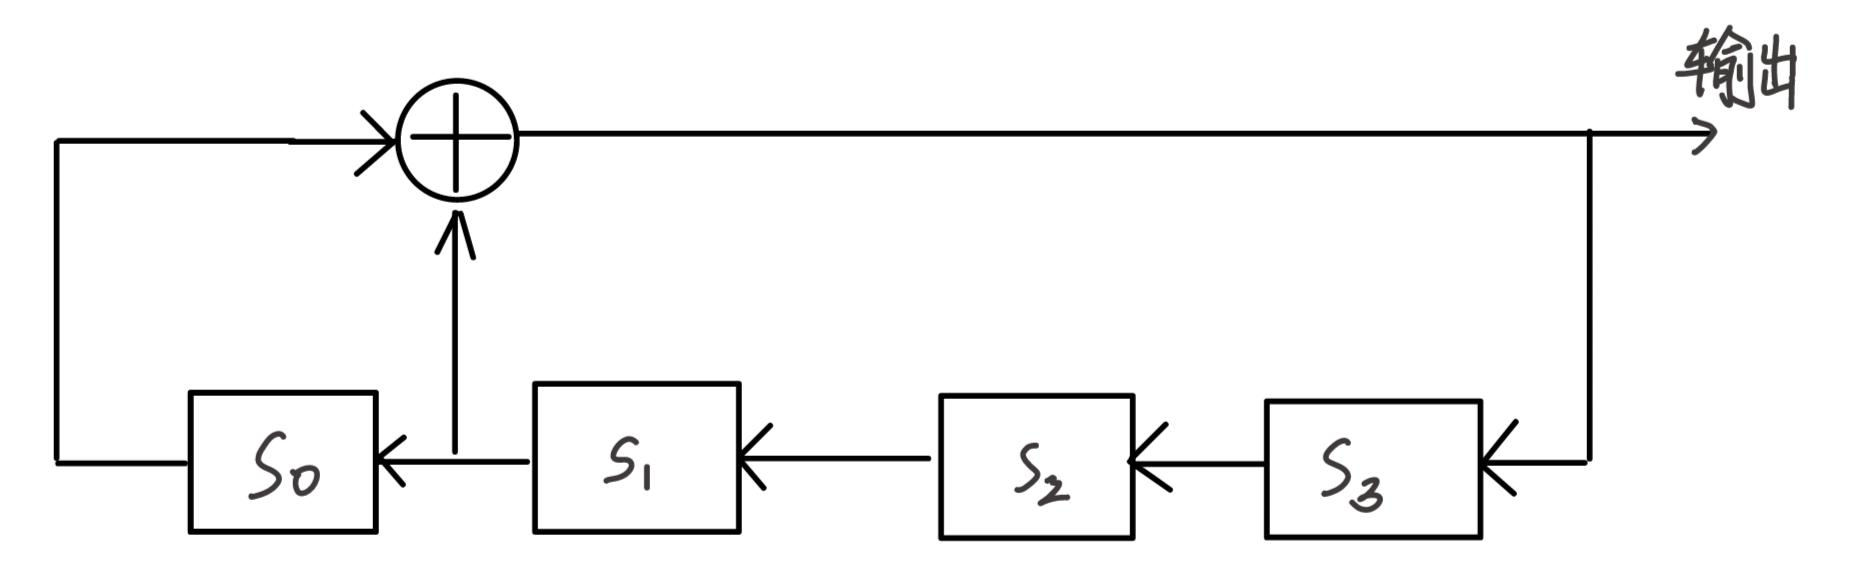
\includegraphics[width=13cm]{线性移位寄存器1.jpg}
        \bottomcaption{\xiaowuhao{线性移位寄存器1}}
      \end{figure}
\newpage
      将寄存器的初值设置为1001,进行运算后得到的状态变迁表如下表所示\par
      \begin{table}[h!]
        \begin{center}
          \caption{序列1状态变迁表}
          \begin{tabular}{c|c|c|c|c} % <-- Now 5 columns
            \textbf{状态序号} & \textbf{S0} & \textbf{S1} & \textbf{S2} & \textbf{S3} \\
            \hline
            1  & 1 & 0 & 0 & 1 \\
            2  & 0 & 0 & 1 & 1 \\
            3  & 0 & 1 & 1 & 0\\
            4  & 1 & 1 & 0 & 1\\
            5  & 1 & 0 & 1 & 0\\
            6  & 0 & 1 & 0 & 1\\
            7  & 1 & 0 & 1 & 1\\
            8  & 0 & 1 & 1 & 1\\
            9  & 1 & 1 & 1 & 1\\
            10 & 1 & 1 & 1 & 0\\
            11 & 1 & 1 & 0 & 0\\
            12 & 1 & 0 & 0 & 0\\
            13 & 0 & 0 & 0 & 1\\
            14 & 0 & 0 & 1 & 0\\
            15 & 1 & 0 & 0 & 1\\
            16 & 1 & 0 & 0 & 1\\
            17 & 0 & 0 & 1 & 1\\
            18 & 1 & 1 & 1 & 0\\
          \end{tabular}
        \end{center}
      \end{table}
      由状态变迁的过程得到的输出序列为101011110001001...,该序列是一个周期为$2^{4}-1=15$的m序列。

    \subsubsection{实验(2)}
      使用本原多项式$g1(x)=x^{4} +x^{3} +1$为连接多项式组成线性移位寄存器。画出逻辑图,写出输出序列及状态变迁。\par
\newpage
      将本原多项式$g1(x)=x^{4} +x^{3} +1$选定为连接多项式得到的线性移位寄存器的逻辑图如下图所示
      \begin{figure}[H]
        \centering
        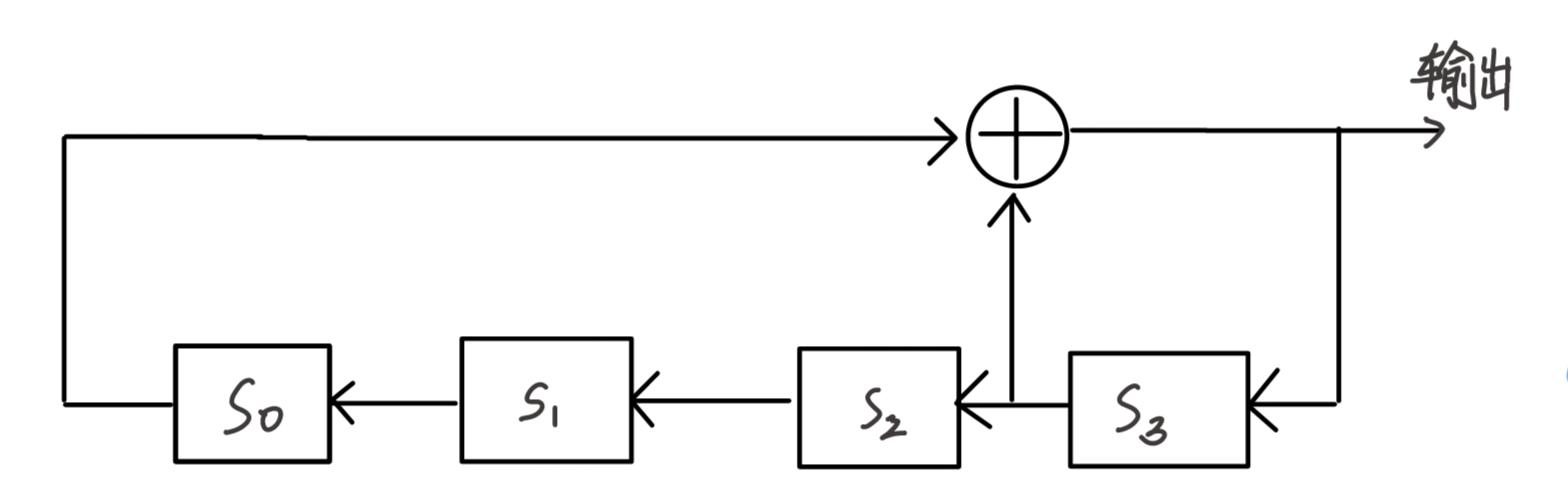
\includegraphics[width=13cm]{线性移位寄存器2.jpg}
        \bottomcaption{\xiaowuhao{线性移位寄存器2}}
      \end{figure}
      将寄存器的初值设置为1001,进行运算后得到的状态变迁表如下表所示\par
      \begin{table}[h!]
        \begin{center}
          \caption{序列2状态变迁表}
          \begin{tabular}{c|c|c|c|c} % <-- Now 5 columns
            \textbf{状态序号} & \textbf{S0} & \textbf{S1} & \textbf{S2} & \textbf{S3} \\
            \hline
            1  & 1 & 0 & 0 & 1 \\
            2  & 0 & 0 & 1 & 0 \\
            3  & 0 & 1 & 0 & 0\\
            4  & 1 & 0 & 0 & 0\\
            5  & 0 & 0 & 0 & 1\\
            6  & 0 & 0 & 1 & 1\\
            7  & 0 & 1 & 1 & 1\\
            8  & 1 & 1 & 1 & 1\\
            9  & 1 & 1 & 1 & 0\\
            10 & 1 & 1 & 0 & 1\\
            11 & 1 & 0 & 1 & 0\\
            12 & 0 & 1 & 0 & 1\\
            13 & 1 & 0 & 1 & 1\\
            14 & 0 & 1 & 1 & 0\\
            15 & 1 & 1 & 0 & 0\\
            16 & 1 & 0 & 0 & 1\\
            17 & 0 & 0 & 1 & 0\\
          \end{tabular}
        \end{center}
      \end{table}
      由状态变迁的过程得到的输出序列为000111101011001...,该序列是一个周期为$2^{4}-1=15$的m序列。

    \subsubsection{输出序列关系}
      对比两组输出序列的关系\\
      提示:(1)与(2)中的多项式是互反多项式,所谓互反多项式是指f(x)与$x^{n} f(\frac{1}{x} )$\par
      (1)中所得的输出序列为101011110001001...,(2)中所得的输出序列为\par
      000111101011001...,将序列1反向输出
      可以得到100100011110101,将序列2调整顺序后将第12位作为周期的首位可得输出序列位100100011110101,与
      序列1反向输出后的结果相同,由此可以得到结果两组输出序列相反,即为互反多项式构成的线性移位寄存器的输出序列
      相反。
      
  \subsection{随机性测试}
    随机性假设测试准则

    \subsubsection{准则1(频率测试)}
      在S的周期SN中,1的个数与0的个数至多相差1。\par
      (1)序列1:\par
      统计序列1一个周期中的1的个数为8,0的个数为7,由于无论周期内的序列顺序如何选取,周期中的1和0的总量
      都不会发生改变,所以可以得出序列1中1的个数与0的个数相差1,满足频率测试\par
      (2)序列2:\par
      统计序列2一个周期中的1的个数为8,0的个数为7由于无论周期内的序列顺序如何选取,周期中的1和0的总量
      都不会发生改变,所以可以得出序列2中1的个数与0的个数相差1,满足频率测试\par

    \subsubsection{准则2(游程测试)}
      在S的周期SN中,至少有1/2的游程长度为1,至少有1/4的游程长度为2,至少有1/8的游程长度为3,以此类推,
      并且0和1游程的个数近似相等。\par
      (1)序列1:\par
        统计序列1的游程长度与数量的关系得到结果如下表所示
        \begin{table}[H]
          \begin{center}
            \caption{序列1游程长度与数量关系}
            \begin{tabular}{c|c|c|c} % <-- Now 5 columns
              \textbf{游程长度} & \textbf{0游程个数} & \textbf{1游程个数} & \textbf{总个数} \\
              \hline
              1  &2&2& 4 \\
              2  &1&1& 2  \\
              3  &1&0& 1 \\
              4  &0&1& 1  \\
            \end{tabular}
          \end{center}
        \end{table}
        游程长度为1的个数为4,占总游程数的比例$\ge \frac{1}{2}$,游程长度为2的个数为2,占总游程数的比例$\ge \frac{1}{4}$
        游程长度为3的个数为1,占总游程数的比例$\ge \frac{1}{8}$,游程长度为4的个数为1,占总游程数的比例$\ge \frac{1}{16}$
        并且0游程与1游程的个数相等,所以序列1满足游程测试。\par

      (2)序列2:\par
        统计序列2的游程长度与数量的关系得到结果如下表所示
        \begin{table}[H]
          \begin{center}
            \caption{序列2游程长度与数量关系}
            \begin{tabular}{c|c|c|c} % <-- Now 5 columns
              \textbf{游程长度} & \textbf{0游程个数} & \textbf{1游程个数} & \textbf{总个数} \\
              \hline
              1  &2&2& 4 \\
              2  &1&1& 2  \\
              3  &1&0& 1 \\
              4  &0&1& 1  \\
            \end{tabular}
          \end{center}
        \end{table}
        游程长度为1的个数为4,占总游程数的比例$\ge \frac{1}{2}$,游程长度为2的个数为2,占总游程数的比例$\ge \frac{1}{4}$
        游程长度为3的个数为1,占总游程数的比例$\ge \frac{1}{8}$,游程长度为4的个数为1,占总游程数的比例$\ge \frac{1}{16}$
        并且0游程与1游程的个数相等,所以序列2满足游程测试。
\newpage
    \subsubsection{准则3(自相关测试)}
      自相关函数R(t)是双值的。即对某个整数K,有:\par
      $N\cdot R(t)=\sum_{i=0}^{N-1}(2s_{i}-1)(2s_{i+t}-1)=\left\{
        \begin{matrix} N,t=0\\K,1\le t\le N-1\end{matrix}\right. $\par
        编写程序验证该公式的程序代码如下所示:
        \lstinputlisting[caption={序列1验证程序},captionpos=b]{E:/Python_code/codes/cryptography/lab_4/Rt.py}
      (1)序列1:\par
        在序列1中输出序列为101011110001001...,且周期N=15,程序的运行结果如下图所示
        \begin{figure}[H]
          \centering
          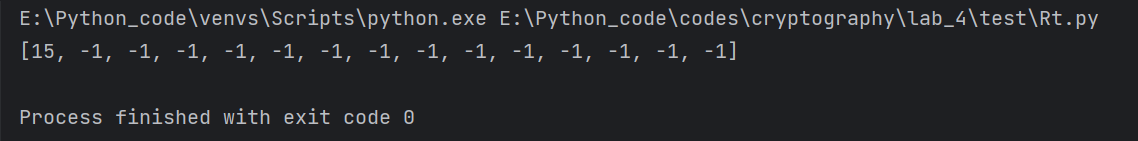
\includegraphics[width=13cm]{Rt_result1.png}
          \bottomcaption{\xiaowuhao{序列1验证结果}}
        \end{figure}
        观察结果可得,整数K为-1,当t为0时公式的结果为N=15,t不为0时程序的运行结果为K=-1,因此序列1满足自相关性测试
        
      (2)序列2:
        在序列1中输出序列为000111101011001...,且周期N=15,程序的运行结果如下图所示
          \begin{figure}[H]
            \centering
            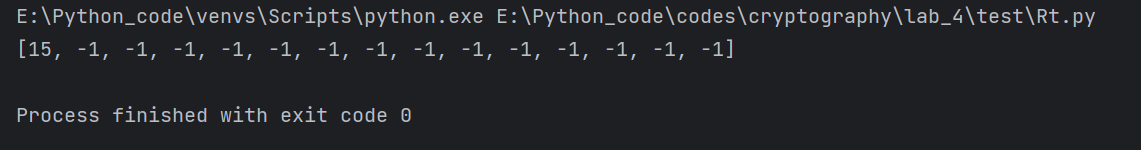
\includegraphics[width=13cm]{Rt_result2.png}
            \bottomcaption{\xiaowuhao{序列2验证结果}}
          \end{figure}
          观察结果可得,整数K为-1,当t为0时公式的结果为N=15,t不为0时程序的运行结果为K=-1,因此序列2满足自相关性测试

  \subsection{编程实现ZUC算法}

    \subsubsection{算法原理}
      祖冲之密码算法在逻辑上分为上中下三层,上层是16级线性反馈移位寄存器(LFSR)、中层是比特重组(BR)、下层是非线性函数(F),
      算法的整体结构如下图所示
      \begin{figure}[H]
        \centering
        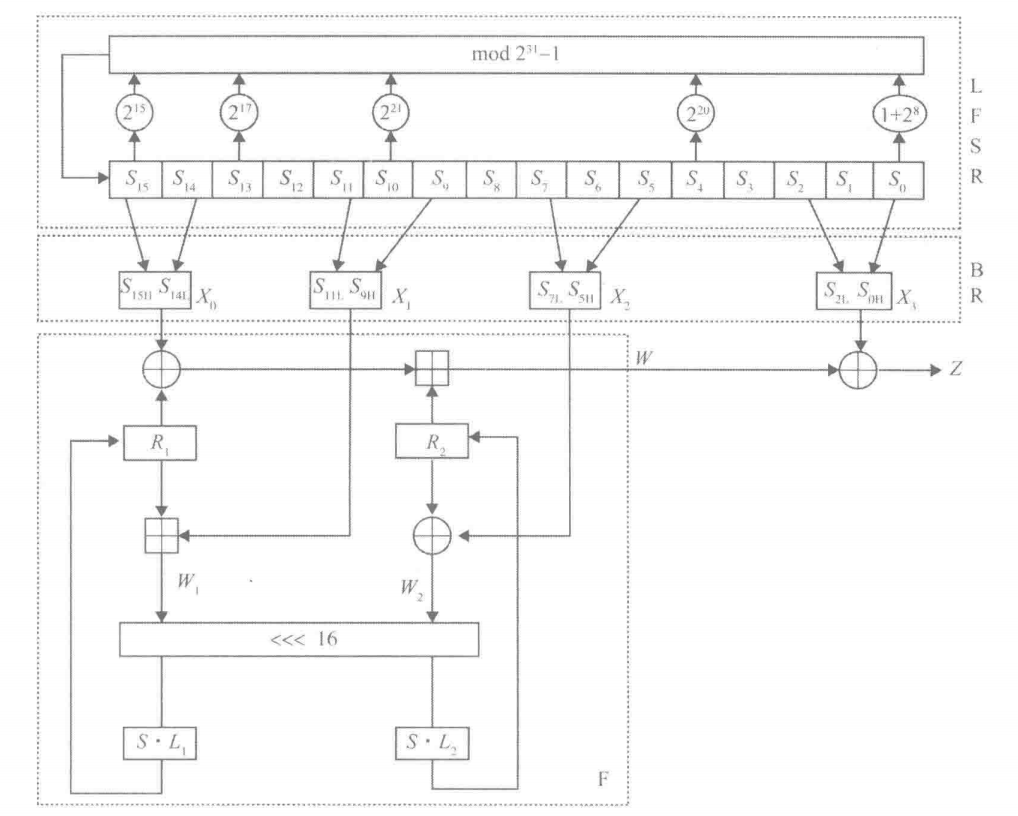
\includegraphics[width=13cm]{ZUC算法结构.png}
        \bottomcaption{\xiaowuhao{祖冲之密码算法结构图}}
      \end{figure}
      (1)线性反馈移位寄存器(LFSR)以一个有限域$GF(2^{31}-1)$上的16次本原多项式为连接多项式,因此,其输出为$GF(2^{31}-1)$上的m序列,
      具有良好的随机性。线性反馈移位寄存器(LFSR)的输出作为中层比特重组(BR)的输入\par
      (2)比特重组(BR)从线性反馈移位寄存器(LFSR)的状态中取出128位,拼凑成4个32位字(X0,X1,X2,X3),供下层的非线性函数F和输出密钥序列使用。\par
      (3)非线性函数(F)从中层的比特重组(BR)接收3个32位字(X0,X1,X2,X3)作为输入,经过内部的异或、循环移位和模$2^{32}$运算,以及两个非线性S盒变换,
      最后输出一个32位字W。由于非线性函数F是祖冲之密码算法中唯一的非线性部件,所以非线性函数F就成为了确保祖冲之密码安全性的关键。\par
      (4)最后,非线性函数F输出的W与比特重组BR输出X3进行异或操作,形成祖冲之密码的输出密钥字序列Z。

    \subsubsection{算法步骤}

      (1)线性反馈移位寄存器:\par
        线性移位寄存器的初始化模式下的程序代码片段如下所示\par
        \lstinputlisting[caption={LFSR初始化模式},captionpos=b,firstline=52,lastline=58]{E:/Python_code/codes/cryptography/lab_4/ZUC/ZUC.py}
        在初始化模式下,LFSR接受一个31比特字u,u是由非线性函数F的32比特输出W通过舍弃最低为比特得到的。\par
        程序首先计算v的值,将S中第15、13、10、4、0项乘对应的系数后与$2^{31}-1$取模。\par
        然后计算$S_{16}$的值,将计算得到的v和输入的U相加后与$2^{31}-1$取模。\par
        然后判断$S_{16}$的值,若其值为0,则将其值置为$2^{31}-1$。\par
        最后将每一项的$S_{i}$的值赋值给其低位$S_{i-1}$。\par
        线性反馈移位寄存器的工作模式下的程序代码片段如下所示
        \lstinputlisting[caption={LFSR工作模式},captionpos=b,firstline=61,lastline=67]{E:/Python_code/codes/cryptography/lab_4/ZUC/ZUC.py}
        在工作模式下相比于初始化模式,程序直接将计算得到的V作为$S_{16}$的值进行之后的操作,其余部分与初始化模式相同,这样的目的在于使得线性反馈移位
        寄存器的状态随机化\par

      (2)比特重组BR:\par
        比特重组部分的程序片段如下所示\par
        \lstinputlisting[caption={比特重组BR},captionpos=b,firstline=70,lastline=75]{E:/Python_code/codes/cryptography/lab_4/ZUC/ZUC.py}
        比特重组部分的作用是从LFSR的寄存器单元中抽取128比特组成4个32比特字X0,X1,X2,X3。其具体的计算过程是将$S_{15}$的高16位与$S_{14}$的低16位进行首尾拼接得到X0;
        然后将$S_{11}$的低16位与$S_{9}$的高16位进行首尾拼接得到X1;然后将$S_{7}$的低16位与$S_{5}$的高16位进行首尾拼接得到X2;
        最后将$S_{2}$的低16位与$S_{0}$的高16位进行首尾拼接得到X3。\par

      (3)非线性函数F\par
        非线性函数F的内部包含2个32bit存储单元R1,R2,F的输入为来自比特重组的三个32bit字X0,X1,X2,输出为一个32bit字W。\par
        非线性函数F的实现代码如下所示
        \lstinputlisting[caption={非线性函数F},captionpos=b,firstline=78,lastline=86]{E:/Python_code/codes/cryptography/lab_4/ZUC/ZUC.py}\par
        该函数首先将输入的X0与其内部的R1进行异或操作然后与R2进行$mod(2^{32})$加法,得到结果W\par
        然后将R1与X1进行$mod(2^{32})$加法,得到结果W1,然后将R2与X2进行异或操作得到W2。\par
        最后将W1的低16位与W2的高16位首尾拼接之后进行比特线性变换1,然后进行S盒变换得到结果R1,
        将W2的低16位与W1的高16位首尾拼接之后进行比特线性变换2,然后进行S盒变换得到结果R2。\par

      (4)S盒变换S\_box\par
        在ZUC算法中的S盒变换由4个并置的8进8出的单个S盒构成,S盒变换接受一个4字节的输入,对于第0、2字节采用S0盒,
        对于第1,3字节采用S1盒,最后输出一个4字节的输出。在单个的S盒中接收一个字节的输入,将字节高位作为行号,
        字节低位作为列号,在S盒表中查找对应项进行输出。\par
        S盒的实现代码如下所示
        \lstinputlisting[caption={S盒变换},captionpos=b,firstline=99,lastline=137]{E:/Python_code/codes/cryptography/lab_4/ZUC/ZUC.py}\par

      (5)32比特线性变换L\par
        线性比特变换的实现代码如下所示
        \lstinputlisting[caption={比特线性变换},captionpos=b,firstline=89,lastline=96]{E:/Python_code/codes/cryptography/lab_4/ZUC/ZUC.py}\par
        线性比特变换接收一个32位操作数X,对X操作的公式如下所示\par
        $L_{1}(x)=X\oplus (X<<<2)\oplus (X<<<10)\oplus (X<<<18)\oplus (X<<<24)$\par
        $L_{2}(x)=X\oplus (X<<<8)\oplus (X<<<14)\oplus (X<<<22)\oplus (X<<<30)$\par

      (6)密钥装入\par
        密钥装入部分的实现代码如下所示
        \lstinputlisting[caption={密钥装入},captionpos=b,firstline=193,lastline=197]{E:/Python_code/codes/cryptography/lab_4/ZUC/ZUC.py}\par
        在密钥装入过程中是将128位的初始密钥KEY和128位的初始向量IV拓展为16个31比特字作为LFSR寄存器单元变量S的初始状态,在每一次拓展中选取KEY中的8位,
        再选取240比特常量D中的15位,最后选取IV中的8位拼凑成S中的一项。

    \subsubsection{算法运行} 
      算法首先进行初始化阶段,执行密钥装入模块将128位的初始密钥KEY和128位的初始向量IV拓展为16个31比特字装入LFSR的寄存器单元变量S中之后作为LFSR的初态
      然后将非线性函数F中的32位存储单元R1和R2置为0,随后重复32次依次进行比特重组、非线性函数变换F和线性反馈移位寄存器LFSR的初始化模式。算法的初始化代码如下所示
      \lstinputlisting[caption={算法初始化阶段},captionpos=b,firstline=140,lastline=151]{E:/Python_code/codes/cryptography/lab_4/ZUC/ZUC.py}\par
      然后算法进入工作阶段,首先依次执行比特重组、非线性函数变换F和线性反馈移位寄存器LFSR之后将F的输出W舍弃,然后进入密钥输出阶段,将比特重组、非线性函数F运行后得到的W与X3异或得到Z、
      LFSR操作定义为一个节拍,每运行一个节拍将Z输出,最后得到的Z即为最终的密钥。算法工作阶段的代码如下所示
      \lstinputlisting[caption={算法工作阶段},captionpos=b,firstline=166,lastline=178]{E:/Python_code/codes/cryptography/lab_4/ZUC/ZUC.py}\par

\newpage
  \subsection{思考与拓展阅读}

    \subsubsection{定理}
      GF(2)上的 n级移位寄存器有$2^{n}$个状态,有$2^{2^{n}}$种不同的反馈函数\par
      对于移位寄存器而言,每一个反馈系数都可以选择0或者1,所以所有的反馈系数都参与排列组合可以有$2^{n}$中组合形式,
      所以也就有$2^{n}$个状态,对于每一个状态的输出都可以映射为0或1,所以不同的反馈函数的数量应为$2^{2^{n}}$

    \subsubsection{定理}
      GF(2)上的 n级移位寄存器中线性反馈函数只有$2^{n-1}$种\par
      若n级线性移位寄存器的系数$g_{n}$为0,则输出反馈不到$S_{n-1}$,因此在实际应用时应该保持其永远为1,所以线性反馈函数
      应该只有$2^{n-1}$种
    \subsubsection{定理}
      n次本原多项式的个数是$\frac{\phi (2^{n}-1)}{n} $ ,其中$\phi $是欧拉函数;(欧拉函数:小于或等于x的数中与x互质的数的数目)
      例如对于n=4,$\frac{\phi (2^{4}-1)}{4}=2 $因此对于4元的线性移位寄存器,只有2个LFSR可以生成m序列,即实验(1)和(2)\par
      一个本原多项式的根在 GF(2) 的扩展域中产生一个周期为$2^{n}-1$的序列。这意味着序列中的元素在达到$2^{n}-1$次幂时第一次回到起点。
      这相当于说,这个周期是与$2^{n}-1$ 互素的所有数的集合\par
      欧拉函数$\phi (2^{n}-1)$给出了与$2^{n}-1$ 互素的数的个数。在本原多项式的上下文中,这表示$2^{n}-1$的周期内不同的状态数量\par
      每个本原多项式在其周期内产生 n个不同的状态(因为它是 n 次的),这些状态是彼此旋转等价的。因此$\phi (2^{n}-1)$给出的是周期内所有不同状态的总数,
      而我们需要将这个数字除以 n,以排除那些由于旋转产生的重复状态。\par
      所以可得 n次本原多项式的个数是$\frac{\phi (2^{n}-1)}{n} $ 
      
    \subsubsection{分析原因}
      在实际的序列密码设计中,人们往往选择项数较少的本原多项式构造LFSR,例如三项式或五项式。试分析选择的原因。\par
      (1)硬件实现的简便性:项数较少的本原多项式意味着更简单的硬件实现。在硬件中,每一个额外的项都需要额外的逻辑门和连接。
          三项式或五项式的本原多项式可以显著减少所需的硬件资源,降低复杂性和成本。\par
      (2)计算效率:在软件实现中,项数较少的多项式意味着更少的计算步骤。
          这在对性能有严格要求的应用中尤其重要,如实时加密通信或大容量数据加密。\par
      (3)可靠的统计性质:尽管本原多项式的项数较少,但如果正确选择,它们仍然可以产生具有良好统计性质的伪随机序列。
          这对于加密应用来说至关重要,因为它保证了序列的不可预测性和均匀分布。\par
      (4)易于分析和验证:简单的本原多项式使得对生成的序列进行数学分析和安全性验证更为容易。
          在密码学中,能够证明加密算法的强度是非常重要的,而复杂的算法往往更难以分析。\par
      (5)抵抗某些攻击的能力:虽然简单的本原多项式可能看起来更容易受到攻击,但如果正确使用,它们可以提供足够的安全性。
          此外,可以通过将多个简单的LFSR结合起来(如在非线性反馈移位寄存器中那样)来提高安全性,而不是增加单个LFSR中的项数。\par
      (6)可调性和灵活性:简单的本原多项式提供了一种在保持硬件和软件效率的同时调整和优化性能的方法。
          例如,通过改变反馈点的位置,可以生成不同的序列,而不需要改变整体设计。\par

    \subsubsection{定理}
      本原多项式一定是不可约多项式;反之则不一定成立。\par

      假设存在一个本原多项式p(x)不是不可约的,即它可以被分解为两个或更多次数较低的多项式的乘积。\par
      由于p(x) 是本原的,其根$\alpha $生成 GF(2) 扩展域的循环群,具有阶$2^{n}-1$\par
      如果p(x)可分解,那么$\alpha $也是这些较低次数多项式的根。这意味着$\alpha $ 的阶必须小于$2^{n}-1$,
      因为较低次数多项式的根的阶最多是它们次数的2的幂减 1。\par
      这与$\alpha $的阶是$2^{n}-1$的事实矛盾。因此,本原多项式p(x)必须是不可约的。\par

      考虑不可约多项式q(x) 在 GF(2) 中的一个根$ \beta $\par
      $ \beta $的阶可能小于$2^{n}-1$。例如,如果$ \beta $的阶是$2^{n}-1$的一个因子,那么q(x)就不是本原的。\par
      因此,尽管q(x) 是不可约的,它并不一定是本原的,因为其根的阶可能不是最大的。

    \subsubsection{常用的判定GF(2)上的不可约多项式的方法}
      (a)如果f(x)的常数项为0,除f(x)=x之外,f(x)一定可约\par
      (b)如果f(x)的项数为偶数,除f(x)=x+1之外,f(x)一定可约\par
      (c)如果f(x)中各项的x的幂次都是2的倍数,f(x)一定可约\par
      (d)如果gcd(f(x), f’(x))≠1,f(x)一定可约\par
      (e)如果f(x+1)可约,f(x)一定可约\par
      (f)如果$ x^{n}f(\frac{1}{x} )$可约,f(x)一定可约\par

      
    \subsubsection{密码设计的初步尝试}
      (a)设计AES类的S盒
      选择不同的不可约多项式,按照AES S盒的相同计算过程即可\par
      按照AES的S盒的计算过程设计S盒的过程如下所示:\par
      1. 选择不可约多项式。假设我们选择一个不同于AES的不可约多项式用于$GF(2^{8})$。
        我们可以选用 $m(x) = x^{8} + x^{6} + x^{5} + x^{2} + 1$。\par
      2. 构建有限域。使用选定的多项式,我们可以构建一个256元素的伽罗瓦域($GF(2^{8})$)。
        在这个域中,每个元素都可以表示为一个多项式,其次数小于8,并且所有的系数都是在GF(2)中,即它们可以是0或1。\par
      3. 定义逆元素。对于域中的每个非零元素,我们需要找到它的乘法逆。这可以通过扩展的欧几里得算法来完成。逆元素是用于后续的仿射变换。\par
      4. 设计仿射变换。仿射变换是一个线性变换加上一个常量偏移。假设我们选择一个简单的线性变换和一个随机的偏移,
        例如,我们可以将每个字节与一个固定的矩阵相乘并加上一个常量向量。\par
      5. 组合所有步骤。最后,我们的S盒将是将每个输入字节映射到其在$GF(2^{8})$中的逆,然后应用我们设计的仿射变换。\par
      (b)生成m序列
      选择不同的本原多项式,按照LFSR的构造过程即可\par
      编写的计算LFSR的程序如下所示
      \lstinputlisting[caption={计算m序列},captionpos=b]{E:/Python_code/codes/cryptography/lab_4/get_m.py}\par
      选定本原多项式为$x^{4}+x+1$运行该程序得到的结果如下图所示
      \begin{figure}[H]
        \centering
        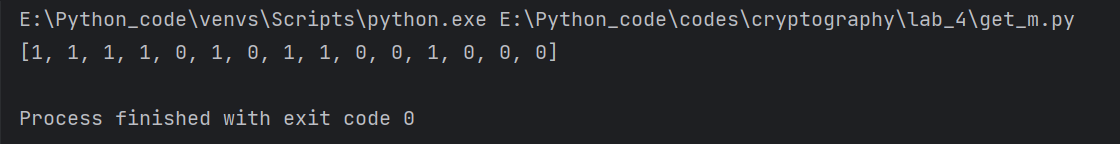
\includegraphics[width=13cm]{get_m_result.png}
        \bottomcaption{\xiaowuhao{计算m序列结果}}
      \end{figure}

    
\section{实验结果与数据处理}
  运行祖冲之代码程序得到的结果如下图所示
  \begin{figure}[H]
    \centering
    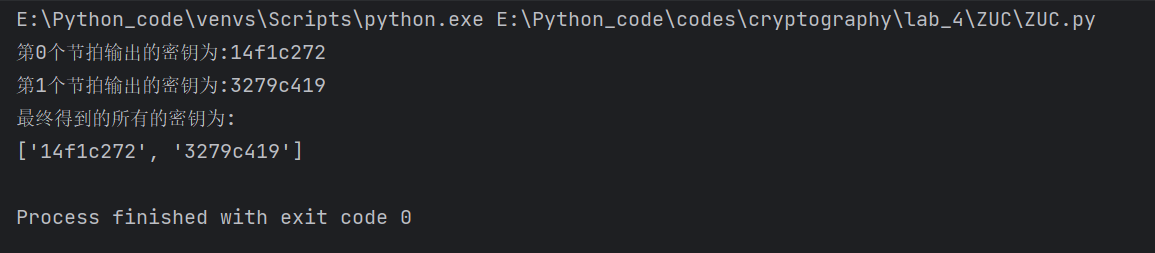
\includegraphics[width=13cm]{ZUC_result.png}
    \bottomcaption{\xiaowuhao{祖冲之密码算法结果}}
  \end{figure}
    
      
\section{分析与讨论}
  (1)通过学习序列密码的基本概念,我更深入地理解了密码学的基础知识,尤其是序列密码在安全通信中的重要性。\par
  (2)实验中,我掌握了线性移位寄存器的构造和操作,这让我了解到伪随机序列在加密中的应用和重要性。\par
  (3)非线性序列的学习让我认识到密码设计的复杂性和创新性。\par
  (4)通过熟悉伪随机性评价方法,我学会了如何评估一个密码算法的安全性。\par
  (5)实现ZUC算法的过程加深了我对流密码实现原理的理解。\par

\section{教师评语}

\end{document}
